\documentclass[10pt,letterpaper]{article}
\usepackage[utf8]{inputenc}
\usepackage[english]{babel}
\usepackage{amsmath}
\usepackage{amsfonts}
\usepackage{amssymb}
\usepackage{graphicx}

\title{Report}
\date{May 18, 2020}
\author{Julio C. Enciso-Alva}



\begin{document}

\maketitle

\section{Dataset}

EEG recordings comes from
`cold pressor' experiment realized on
a single subject (identified as `Peng') on one single session. 
%Experiment consists on a single session. 
Cold pressor experiment consist on the subject sitting on a chair;
as stimuli, subject's left/right hand is submerged 
in warm/cold water for 1 minute. Both hands are kept on the air  for 5 minutes between stimuli. 
Multiple stimuli are presented on the following sequence:
\begin{enumerate}
	\item Right hand, warm water.
	\item Right hand, cold water.
	\item Left hand, warm water.
	\item Left hand, cold water.
\end{enumerate}
The sequence is repeated 3 times, making a total of 12 trials.

EEG was recorded at 1 kHz from 61 electrodes located according to the International 10\% System (Fig \ref{fig:electrodes}). 

For the reconstruction, observation windows consider only 6 sec before and 20 sec within each stimuli.

\begin{figure}
\centering
	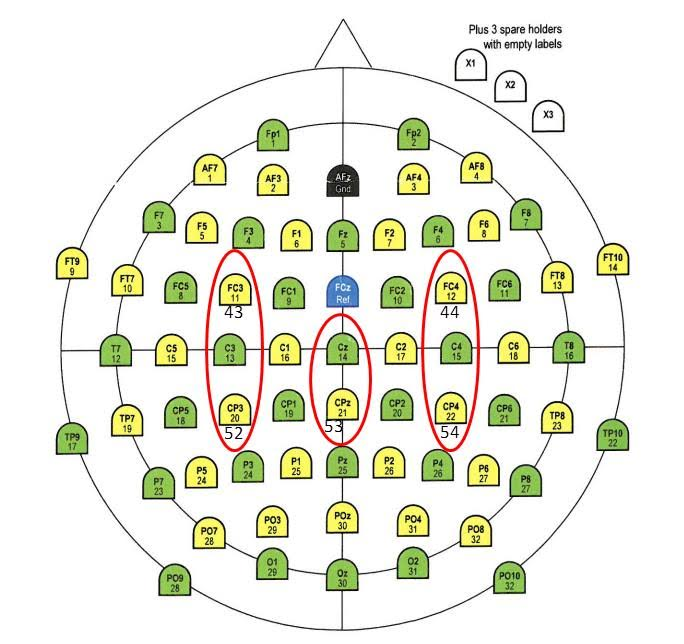
\includegraphics[width=0.6\linewidth]{easycap_layout_peng}
	\caption{Location of electrodes, according to the 10\% International System with 3 reference electrodes.
	Colors indicate that 64-electrode recording was achieved by simultaneous use of two 32-channel
	amplifiers. Figure by Dr. Hongguang Xi.}
	\label{fig:electrodes}
\end{figure}

\section{Source reconstruction using Fieldtrip}

Fieldtrip 20200227 was utilized for EEG data processing. 
Geometry for head, skull and head were provided by Dr. Hongguang Xi.

On a first moment, source reconstruction was performed using Minimum Norm Estimate (MNE).
In particular it was used the implementation already included in Fieldtrip by Oostenveld (2008).

After the source reconstruction was performed, a 3 sec moving-average was applied to the data.
Data was projected into brain surface for visualization, as shown in Figure \ref{fig:sample}.

\begin{figure}
\centering
	\includegraphics[width=\linewidth]{trial03_sample}
	\caption{(Up) EEG registers on a sample observation window at trial 3: left hand, warm water.
	Time $t=0$ is set to start of stimulus. (Down) After electrical sources were reconstructed,
	data was smoothed using a 3 sec moving average. 
	Resulting data was projected to the brain surface at $t=[-6,-3], [-5,-2], \dots$.}
	\label{fig:sample}
\end{figure}

\end{document}